\section{目的與規格對照}
依 Lab 13（PDF 第 55--57 頁）比較靜態 CMOS 與偽 NMOS 反相器。步驟 1 保留 500 MHz 輸入並掃描 PMOS/NMOS 寬度比；步驟 2 改變尺寸與負載，量測最高可用頻率區間及其平均功率。另以 DC 掃描分離低準位誤差與靜態耗電。四個 netlist 共 116 個變體全部完成求解與量測。

\section{電路與判定方法}
兩種電路均以 NMOS 作下拉；CMOS 的 PMOS gate 接輸入，偽 NMOS 的 PMOS gate 固定為 0，使其持續導通。基準尺寸為 $W_n=0.6\,\mu$m、$W_p=0.9\,\mu$m、$L=0.25\,\mu$m，負載 7 fF。寬度比掃描 0.25/0.5/1/1.5/3/6；尺寸／負載比較採 (1 倍,7 fF)、(2 倍,7 fF)、(1 倍,14 fF)、(2 倍,14 fF)。

本次以固定且明示的邏輯判準定義可用頻率：穩定後的低準位取樣值不超過 0.3 V、高準位不低於 0.7 V。先掃描 0.1--10 GHz，再把通過／不通過之間細化至 0.1 GHz。這是該取樣位置與負載下的頻率區間，不是所有接收器皆適用的元件額定頻率，也不是連續頻率軸上的精確最大值。

\section{模擬設定與量測定義}
本次使用獨立提供的 MOS 模型，電源為 1.0 V、溫度為 $27\,^{\circ}$C，並保留講義的電路拓樸及下列比較條件。1 V 是本次模擬設定，並非由公開模型文件確認的元件額定值；不能把講義舊製程的數值當成此次模型的驗收值。

模擬使用 HSPICE S-2021.09、RUNLVL=6。表格取自實際原生量測結果，圖形由實際列印數據重繪；每個變體都完整重設掃描參數及溫度，避免前一個變體的設定殘留。數值求解完成與量測成功，不等於已驗證製程可靠度。加密模型區塊的內部警告仍無法完整檢視。
輸入每週期在 $0.25T$ 開始上升，rise/fall 參數各為 $0.01T$、高準位脈寬 $0.48T$；暫態共 12 週期，每週期列印 500 點。低準位在 $10.7T$、高準位在 $11.2T$ 取樣；功率對第 4 至第 12 週期積分平均。兩種電路使用獨立理想供應源，以 $P=-\overline{V_{DD}I(V_{DD})}$ 取得正的供應功率。

\section{寬度比與靜態結果}
下表為 500 MHz、尺寸 1、7 fF；功率單位為 $\mu$W。

\begin{center}\small
\begin{tabular}{llllll}
\toprule
$W_p/W_n$ & CMOS $V_L$ & Pseudo $V_L$ & Pseudo $V_H$ & CMOS P & Pseudo P \\
\midrule
0.25 & 0.0000 & 0.0110 & 0.8140 & 3.700 & 7.823 \\
0.5 & 0.0000 & 0.0232 & 0.9910 & 4.441 & 12.783 \\
1 & 0.0000 & 0.0485 & 1.0000 & 4.810 & 21.706 \\
1.5 & 0.0000 & 0.0755 & 1.0000 & 5.156 & 30.540 \\
3 & 0.0000 & 0.1709 & 1.0000 & 6.138 & 56.405 \\
6 & 0.0000 & 0.5860 & 1.0000 & 7.918 & 92.040 \\
\bottomrule
\end{tabular}
\end{center}
\begin{figure}[htbp]
\centering
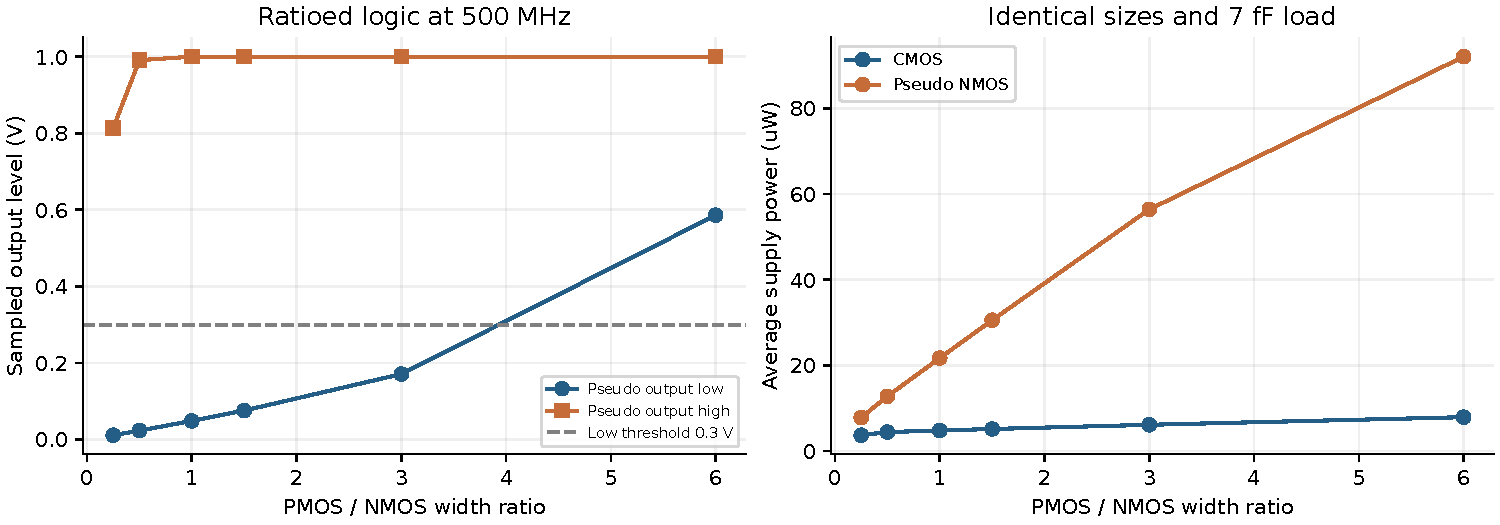
\includegraphics[width=\linewidth]{figures/pseudo_ratio.pdf}
\caption{持續上拉造成準位與功率對寬度比敏感；比值 6 的低準位不合格。}
\end{figure}
DC 輸入為 1 V 時，CMOS 輸出為 3.88 $\mu$V；偽 NMOS 為 0.07550 V，靜態供應電流為 54.548 $\mu$A。該電流是輸出被持續拉低時的值；平均靜態功率還要乘上相應輸入停留比例。
\section{最高通過頻率與功率}
下界為通過點，上界為相鄰不通過點；功率取下界實測值。

\begin{center}\small
\begin{tabular}{lllll}
\toprule
Size & Load (fF) & Logic & Pass / fail (GHz) & P ($\mu$W) \\
\midrule
1 & 7 & CMOS & 3.0 / 3.1 & 25.302 \\
1 & 7 & Pseudo NMOS & 3.8 / 3.9 & 50.583 \\
2 & 7 & CMOS & 4.5 / 4.6 & 50.934 \\
2 & 7 & Pseudo NMOS & 6.0 / 6.1 & 101.683 \\
1 & 14 & CMOS & 1.8 / 1.9 & 24.942 \\
1 & 14 & Pseudo NMOS & 2.2 / 2.3 & 50.658 \\
2 & 14 & CMOS & 3.0 / 3.1 & 50.741 \\
2 & 14 & Pseudo NMOS & 3.8 / 3.9 & 101.784 \\
\bottomrule
\end{tabular}
\end{center}
\begin{figure}[htbp]
\centering
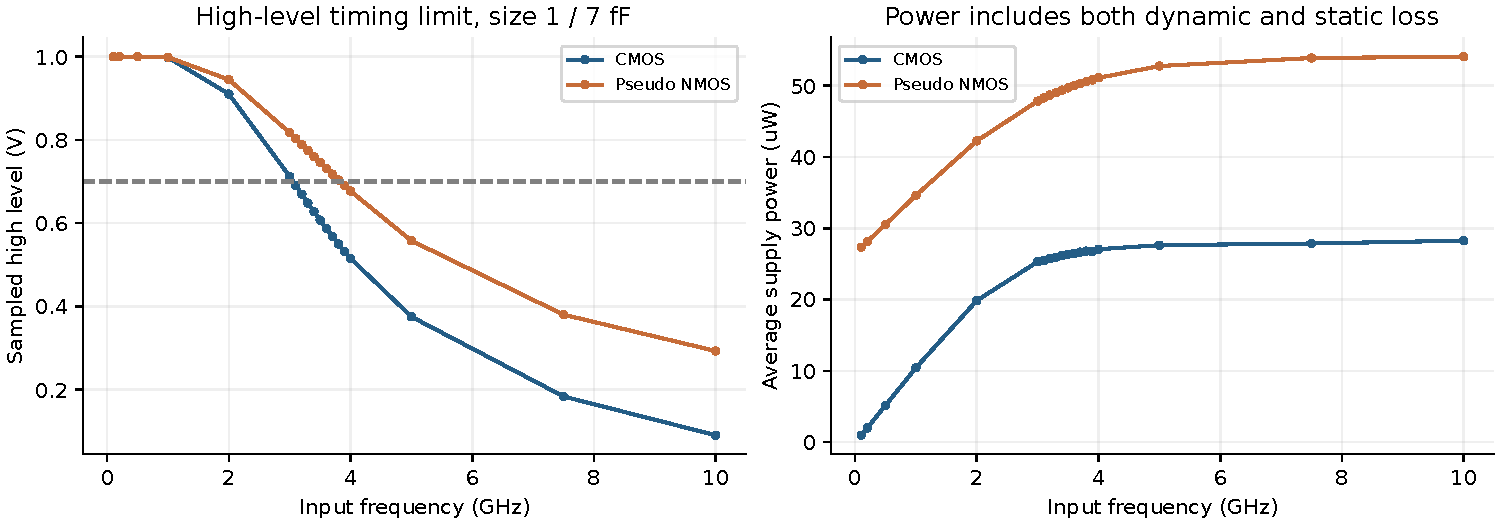
\includegraphics[width=\linewidth]{figures/pseudo_frequency.pdf}
\caption{尺寸 1、7 fF 的輸出高準位與平均功率；不合格頻率點仍保留以顯示失效。}
\end{figure}
\section{討論與問題回答}
尺寸 1、7 fF 時，CMOS 通過到 3.0 GHz、3.1 GHz 不通過；偽 NMOS 通過到 3.8 GHz、3.9 GHz 不通過。加大尺寸可提高這個範圍，但也提高持續導通的電流；加倍負載則降低可用頻率。這個比較同時保留低準位與高準位判準，沒有因為偽 NMOS 擺幅較小就直接把任何小訊號擺動視為可用邏輯。

對每週期一次充放電的近似，CMOS 動態功率為 $fCV_{DD}^{2}$；偽 NMOS 約為 $fCV_{DD}V_{swing}+\overline{I_{DC}}V_{DD}$。因此忽略其他項時，偽 NMOS 較省電的必要比較條件為 $\overline{I_{DC}}<fC(V_{DD}-V_{swing})$。這只是條件式，不保證高頻一定較省電。本次相同尺寸／負載下偽 NMOS 功率較大；超過邏輯判準後，功率趨平也不能稱為有效操作下的節能。

對二輸入 NAND/NOR，靜態 CMOS 各使用 4 個核心電晶體，偽 NMOS 使用 3 個；一般 n 輸入形式則約為 $2n$ 與 $n+1$，但實際面積仍取決於寬度、接點與佈線，這裡沒有版圖面積結論。偽 NMOS 的每個邏輯輸入只驅動下拉網路，可降低前級輸入負載；代價是 DC 通路、較高低準位及比例依賴。NAND 的串聯 NMOS 下拉在最差路徑仍須勝過常開 PMOS；NOR 可用單一 PMOS 取代串聯 PMOS 上拉，但高準位恢復速度仍受該上拉強度限制。以上為電路結構分析，並未另外宣稱 NAND/NOR 的實測速度排名。

\section{可重現檔案}
本實驗上傳下列 netlist；模型設定以註解標記保留，模型檔與其路徑均不隨報告上傳。執行前須在本機補入合法可用的模型設定。
\begin{itemize}
\item \texttt{01\_ratio.sp}
\item \texttt{02\_frequency.sp}
\item \texttt{03\_dc\_power.sp}
\item \texttt{04\_frequency\_refinement.sp}
\end{itemize}
每一個變體的完整量測值位於本 lab 的 \texttt{results}，並附代表性波形 CSV、分析結果與規格對照清單。波形 CSV 最多保留 2501 個均勻取樣點；直接量測未降採樣。完整原始 listing 留在本機。

